\documentclass{article}

% NeurIPS 2025 style
\usepackage[preprint]{neurips_2025}

\usepackage[utf8]{inputenc}
\usepackage[T1]{fontenc}
\usepackage{hyperref}
\usepackage{url}
\usepackage{booktabs}
\usepackage{amsfonts}
\usepackage{amsmath}
\usepackage{amssymb}
\usepackage{nicefrac}
\usepackage{microtype}
\usepackage{xcolor}
\usepackage{graphicx}
\usepackage{listings}
\usepackage{algorithm}
\usepackage{algorithmic}
\usepackage{multirow}
\usepackage{subcaption}
\usepackage{tikz}
\usetikzlibrary{shapes,arrows,positioning,fit,backgrounds}

\lstset{
  basicstyle=\ttfamily\footnotesize,
  breaklines=true,
  frame=single,
  language=TypeScript,
  commentstyle=\color{gray},
  keywordstyle=\color{blue},
  stringstyle=\color{red},
  numbers=left,
  numberstyle=\tiny\color{gray},
  numbersep=5pt
}

\title{%
  \textbf{Inside Claude Code: A Technical Analysis of an Agentic Coding Assistant}\\
  \large Architecture, Tool Orchestration, and Context Management in Production LLM Agents
}

\author{%
  Anonymous Authors\\
  \textit{Under Review}
}

\begin{document}

\maketitle

\begin{abstract}
Large language model (LLM)-based coding assistants have rapidly advanced from simple autocompletion systems to fully autonomous agents capable of multi-step software engineering tasks. Claude Code, Anthropic's command-line coding agent, represents a mature production system embodying a range of novel engineering decisions. In this paper, we present a systematic technical analysis of Claude Code v2.1.88 based on its decompiled source code, comprising 1,332 TypeScript files and approximately 163,000 lines of code. We identify and analyze five core architectural contributions: (1) a \emph{streaming agentic loop} that groups API turns rather than user turns and employs ordered-buffering for concurrent tool execution; (2) a \emph{three-tier hierarchical context management} strategy combining persistent session memory, reactive auto-compaction, and micro-compaction; (3) a \emph{multi-layer permission architecture} integrating static rule matching, ML-based Bash risk classification, and interactive user dialogs; (4) a \emph{Coordinator/Worker multi-agent orchestration} pattern with isolated execution contexts; and (5) a \emph{Model Context Protocol (MCP) integration layer} that unifies first- and third-party tools under a single schema. Our analysis reveals design patterns with broad applicability to future agentic systems, including circuit-breaker mechanisms for context overflow, memory-first compaction strategies, and concurrency models balancing throughput against API ordering semantics. We discuss implications for the design of robust, production-grade LLM agents.
\end{abstract}

% ─────────────────────────────────────────────────────────────
\section{Introduction}
% ─────────────────────────────────────────────────────────────

The emergence of LLM-based agents capable of autonomously executing multi-step software engineering tasks marks a significant inflection point in AI-assisted development~\cite{chen2021evaluating,yao2022react,shinn2023reflexion}. Unlike earlier systems that treated code generation as a single-shot completion problem, modern coding agents maintain persistent state, invoke external tools, manage long conversational contexts, and coordinate multiple sub-agents --- all within a single interactive session.

Academic work has extensively studied the \emph{reasoning} capabilities of such agents~\cite{wei2022chain,yao2022react,park2023generative}, but comparatively little attention has been paid to the \emph{engineering architecture} that enables them to function reliably in production at scale. Questions such as how to handle context overflow gracefully, how to safely orchestrate concurrent tool executions, how to mediate between autonomous action and human oversight, and how to compose heterogeneous tool ecosystems remain largely unexplored in the academic literature.

Claude Code~\cite{anthropic2024claudecode} provides a rare opportunity to study these questions through the lens of a production system. Released by Anthropic as a CLI-based coding agent, its v2.1.88 source code (made available through npm package decompilation) exposes the concrete engineering decisions made to address each of these challenges.

\paragraph{Contributions.} This paper makes the following contributions:
\begin{itemize}
  \item We present the first systematic architectural analysis of a production LLM coding agent based on its actual source code.
  \item We identify and formalize five key architectural patterns: streaming agentic loop, three-tier context management, multi-layer permission architecture, Coordinator/Worker orchestration, and MCP integration.
  \item We abstract design principles from these patterns that are broadly applicable to the construction of production agentic systems.
  \item We discuss open problems and future research directions motivated by the architectural choices observed.
\end{itemize}

% ─────────────────────────────────────────────────────────────
\section{Background and Related Work}
% ─────────────────────────────────────────────────────────────

\subsection{LLM Agents and Tool Use}

The ReAct framework~\cite{yao2022react} popularized the idea of interleaving chain-of-thought reasoning with tool-use actions in a \textsc{Thought-Action-Observation} loop. Subsequent work explored tool selection~\cite{schick2023toolformer}, multi-step planning~\cite{wang2023plan}, and reflection~\cite{shinn2023reflexion}. Toolformer~\cite{schick2023toolformer} demonstrated that LLMs can learn to invoke APIs self-supervised. More recent systems such as AutoGPT~\cite{autogpt2023}, BabyAGI~\cite{nakajima2023babyagi}, and LangChain~\cite{langchain2022} built agent frameworks on top of these ideas, though they largely remain research prototypes.

In the coding domain, Devin~\cite{cognition2024devin}, SWE-agent~\cite{yang2024sweagent}, and OpenHands~\cite{wang2024openhands} have demonstrated autonomous issue resolution. However, these systems focus primarily on benchmark performance and their internal engineering details are not publicly disclosed.

\subsection{Context Window Management}

A fundamental challenge for LLM agents is the finite context window. \citet{liu2023lost} showed that LLMs struggle to attend to information in the middle of long contexts. Retrieval-augmented generation (RAG)~\cite{lewis2020retrieval} addresses this for knowledge retrieval, but not for conversational history. \citet{zhang2024survey} survey summarization-based approaches to conversation compression. Claude Code's three-tier strategy introduces a novel \emph{session memory extraction} approach that we analyze in detail.

\subsection{Multi-Agent Systems}

Multi-agent LLM systems have gained significant interest~\cite{park2023generative,wu2023autogen,hong2023metagpt}. AutoGen~\cite{wu2023autogen} proposes a framework for conversable agents with code execution. MetaGPT~\cite{hong2023metagpt} assigns specialized roles (product manager, architect, developer) to different agents. Claude Code's Coordinator/Worker pattern represents a principled instance of hierarchical multi-agent orchestration with explicit isolation guarantees.

\subsection{Safety and Permission Systems in Agents}

Permission and safety architecture for autonomous agents remains underexplored. \citet{ruan2023identifying} identify risks in LLM tool-use, and \citet{shi2024ehragent} discuss safety in medical agents. Claude Code provides a multi-layer implementation that integrates ML-based risk classification with human-in-the-loop confirmation, offering a concrete reference design.

% ─────────────────────────────────────────────────────────────
\section{System Overview}
% ─────────────────────────────────────────────────────────────

\subsection{Codebase Characteristics}

Claude Code v2.1.88 comprises 1,332 TypeScript source files organized into 11 top-level subsystems (Table~\ref{tab:subsystems}). The codebase is compiled using Bun and targets Node.js $\geq$ 18 as a single bundled executable. The largest single file, \texttt{query.ts}, is approximately 785KB (roughly 18,000 lines after formatting), reflecting the complexity of the core agentic loop. The UI layer uses React rendered via Ink~\cite{ink2023} for terminal output.

\begin{table}[t]
\centering
\caption{Claude Code subsystem organization and scale.}
\label{tab:subsystems}
\small
\begin{tabular}{llrl}
\toprule
\textbf{Subsystem} & \textbf{Directory} & \textbf{Files} & \textbf{Primary Responsibility} \\
\midrule
Query Engine  & \texttt{src/} (root) & 12 & Agentic loop, session state \\
Tools         & \texttt{src/tools/} & 44 dirs & Tool implementations (40+) \\
Services      & \texttt{src/services/} & 22 dirs & Business logic (compact, MCP, \ldots) \\
Commands      & \texttt{src/commands/} & 87 files & Slash command implementations \\
Components    & \texttt{src/components/} & 33 dirs & React/Ink terminal UI \\
Utilities     & \texttt{src/utils/} & 30+ files & Permissions, tokens, hooks \\
State         & \texttt{src/state/} & 8 files & Application state management \\
Bridge        & \texttt{src/bridge/} & 6 files & Desktop/remote bridge \\
Coordinator   & \texttt{src/coordinator/} & 4 files & Multi-agent coordination \\
Assistant     & \texttt{src/assistant/} & stubs & KAIROS autonomous mode \\
Tasks         & \texttt{src/tasks/} & 5 files & Persistent task management \\
\bottomrule
\end{tabular}
\end{table}

\subsection{Execution Modes}

Claude Code operates in four distinct modes: (1) \textit{Interactive CLI} mode, the primary mode where users type requests in a REPL; (2) \textit{Headless/SDK} mode, where the agent is driven programmatically via \texttt{QueryEngine}; (3) \textit{Remote} mode, where the agent runs on a remote machine and communicates over SSH or Teleport; and (4) \textit{Desktop Bridge} mode, connecting to the Claude Desktop application. The architectural analysis in this paper focuses primarily on Interactive CLI and Headless/SDK modes as they expose the core agentic mechanisms.

% ─────────────────────────────────────────────────────────────
\section{The Streaming Agentic Loop}
% ─────────────────────────────────────────────────────────────

\subsection{Architecture Overview}

The central execution engine is implemented in \texttt{src/QueryEngine.ts} (1,295 lines) with the agentic loop itself in \texttt{src/query.ts}. Unlike simpler agent implementations that treat each user message as an independent query, Claude Code maintains a stateful session that accumulates conversation history, file caches, usage statistics, and interrupt signals across the lifetime of an interactive session.

\begin{figure}[t]
\centering
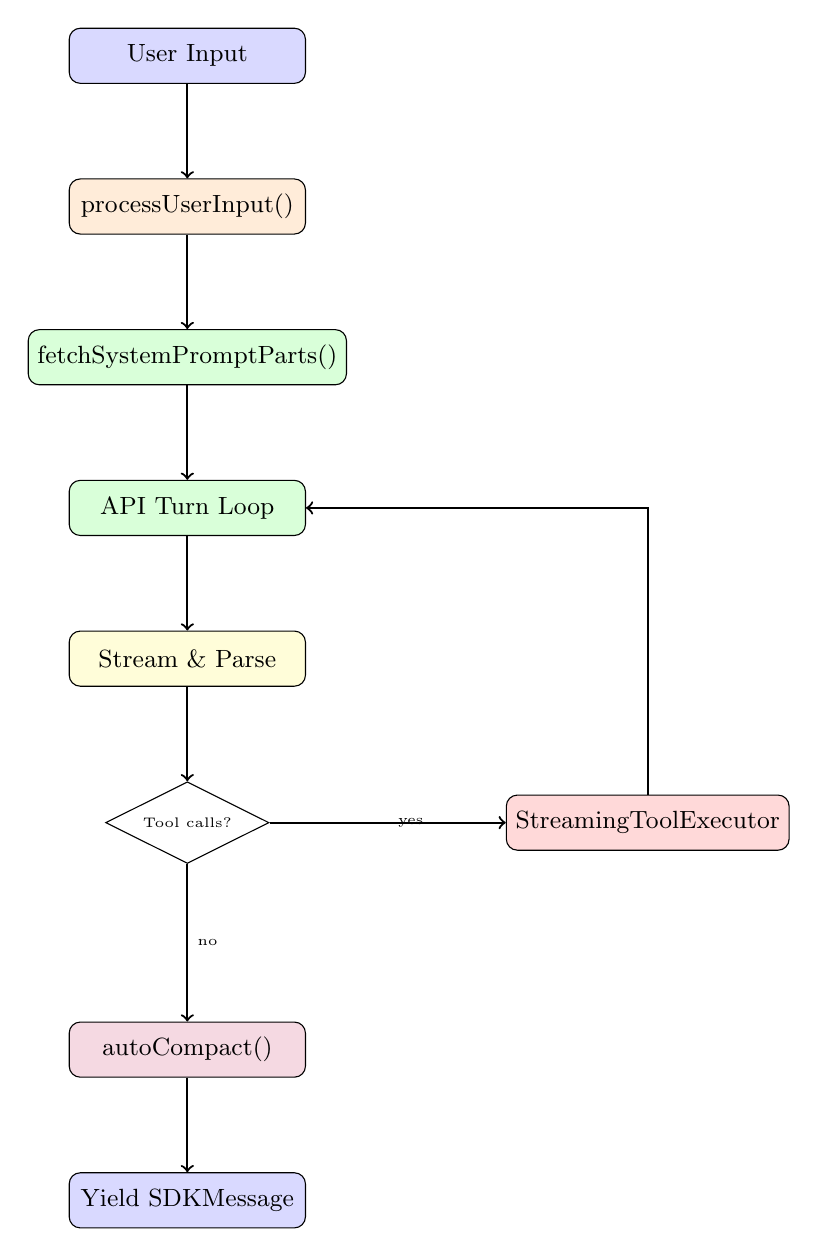
\begin{tikzpicture}[
  node distance=1.2cm,
  box/.style={rectangle, draw, rounded corners, minimum width=3cm, minimum height=0.7cm, text centered, font=\small},
  decision/.style={diamond, draw, minimum width=2cm, minimum height=0.7cm, text centered, font=\tiny, aspect=2},
  arrow/.style={->, thick}
]
\node[box, fill=blue!15] (input) {User Input};
\node[box, fill=orange!15, below=of input] (preproc) {processUserInput()};
\node[box, fill=green!15, below=of preproc] (sysprompt) {fetchSystemPromptParts()};
\node[box, fill=green!15, below=of sysprompt] (apiloop) {API Turn Loop};
\node[box, fill=yellow!15, below=of apiloop] (stream) {Stream \& Parse};
\node[decision, below=of stream] (toolcall) {Tool calls?};
\node[box, fill=red!15, right=3cm of toolcall] (executor) {StreamingToolExecutor};
\node[box, fill=purple!15, below=2cm of toolcall] (compact) {autoCompact()};
\node[box, fill=blue!15, below=of compact] (output) {Yield SDKMessage};

\draw[arrow] (input) -- (preproc);
\draw[arrow] (preproc) -- (sysprompt);
\draw[arrow] (sysprompt) -- (apiloop);
\draw[arrow] (apiloop) -- (stream);
\draw[arrow] (stream) -- (toolcall);
\draw[arrow] (toolcall) -- node[right, font=\tiny]{yes} (executor);
\draw[arrow] (executor) |- (apiloop);
\draw[arrow] (toolcall) -- node[right, font=\tiny]{no} (compact);
\draw[arrow] (compact) -- (output);
\end{tikzpicture}
\caption{The Claude Code streaming agentic loop. API turns (not user turns) drive the inner loop; tool results feed back as new API turns until the model produces a terminal response.}
\label{fig:agentic-loop}
\end{figure}

\subsection{API Turn vs.\ User Turn Grouping}

A key design decision in Claude Code is that the inner loop iterates over \emph{API turns} rather than \emph{user turns}. Each API turn corresponds to one request-response pair with the Claude API. When the API response contains tool calls, these are executed and their results are appended to the message history as a new \texttt{tool\_result} block, which immediately triggers the next API turn without waiting for user input. This continues until the model produces a response containing no tool calls.

This design decouples the user interaction cadence from the LLM inference cadence, enabling complex multi-step tasks within a single ``user turn'' that may internally involve dozens of API turns. The \texttt{QueryEngine} exposes this through the \texttt{submit\_message()} interface, which does not return until the entire agentic trajectory completes.

\subsection{Streaming and Ordered Buffer}

Claude Code uses the Anthropic streaming API (\texttt{stream: true}) and processes events incrementally. The \texttt{StreamingToolExecutor} (519 lines) implements a critical invariant: \textbf{tool results are returned to the API in the order that tool calls were received}, regardless of the actual completion order of concurrent tools.

This is implemented via a result buffer keyed by tool call position index. Concurrent-safe tools (e.g., \texttt{FileReadTool}, \texttt{GlobTool}, \texttt{WebFetchTool}) are dispatched in parallel, but results are enqueued and flushed in FIFO order. Non-concurrent tools (e.g., \texttt{BashTool}, \texttt{FileEditTool}) acquire an exclusive lock before execution. Algorithm~\ref{alg:streaming} formalizes this protocol.

\begin{algorithm}[t]
\caption{Ordered Concurrent Tool Execution}
\label{alg:streaming}
\begin{algorithmic}[1]
\REQUIRE Tool calls $\mathcal{T} = [t_1, t_2, \ldots, t_n]$ from API response
\STATE Initialize ordered buffer $B = [\texttt{null}] \times n$
\STATE Initialize exclusive lock $L$
\FOR{each $t_i \in \mathcal{T}$ (in parallel if $t_i.\texttt{concurrent} = \text{true}$)}
  \IF{$t_i.\texttt{concurrent} = \text{false}$}
    \STATE Acquire $L$
  \ENDIF
  \STATE $r_i \leftarrow \texttt{execute}(t_i)$
  \STATE $B[i] \leftarrow r_i$
  \IF{$t_i.\texttt{concurrent} = \text{false}$}
    \STATE Release $L$
  \ENDIF
\ENDFOR
\STATE \textbf{return} $B$ in index order \COMMENT{Preserves API ordering semantics}
\end{algorithmic}
\end{algorithm}

\paragraph{Sibling abort on Bash error.} Each set of concurrent tool calls shares a \texttt{siblingAbortController}. If \texttt{BashTool} returns a non-zero exit code, it signals this controller, causing all sibling tool executions to abort. This prevents wasted computation and avoids cascading failures in multi-tool turns.

\subsection{System Prompt Construction}

The system prompt is assembled dynamically per API turn by \texttt{fetchSystemPromptParts()}, which composes modular prompt sections. The assembly follows a priority order:
\[
\text{Override} \succ \text{Coordinator} \succ \text{Agent-specific} \succ \text{Custom (user)} \succ \text{Default}
\]
Prompt sections include: agent identity description, tool reference documentation, current permission mode, user-provided context (CLAUDE.md files discovered via directory traversal), and system-injected context (platform, date, working directory). CLAUDE.md discovery traverses upward from the current working directory to the filesystem root, accumulating context at each level, providing hierarchical project-level and organization-level instructions.

% ─────────────────────────────────────────────────────────────
\section{Three-Tier Context Management}
% ─────────────────────────────────────────────────────────────

\subsection{The Context Overflow Problem}

Long-running agentic sessions accumulate extensive message histories. The Anthropic API imposes a hard limit on context length; exceeding this limit results in an HTTP 413 error. Naive truncation risks losing critical information (e.g., original task instructions, earlier tool outputs). Claude Code implements a three-tier strategy to manage this gracefully.

\subsection{Tier 1: Session Memory Extraction}

The first tier proactively extracts \emph{session memory} from the current conversation as it grows. This is implemented as a background forked agent that is triggered when the message history exceeds a configurable threshold ($\approx$60\% of context capacity). The extraction agent receives the conversation history and produces a structured memory document containing:
\begin{itemize}
  \item Task description and current status
  \item Decisions made and their rationale
  \item Code artifacts created or modified
  \item Key facts discovered about the codebase
\end{itemize}

The extracted memory is stored in \texttt{\textasciitilde/.claude/projects/[project-hash]/memory/} and automatically loaded at session resumption. Crucially, this extraction runs \emph{asynchronously} without blocking the main agent loop --- a ``memory-first'' strategy that prioritizes low-latency extraction over completeness.

\subsection{Tier 2: Auto-Compaction}

The second tier, \texttt{autoCompact()} in \texttt{src/services/compact/autoCompact.ts}, is triggered when the context approaches the hard limit and Tier 1 has not yet sufficiently reduced it. It implements three compaction strategies, applied in order:

\paragraph{(a) Session memory replacement.} If an existing session memory document is available, the message history between the last compaction point and the present is summarized and the memory document is updated. The original messages are then truncated.

\paragraph{(b) Reactive compaction.} A dedicated compaction agent processes the full message history and produces a compressed summary that preserves the most relevant information. The original history is replaced with: [COMPACTED SUMMARY] + current turn context.

\paragraph{(c) Micro-compaction.} For histories that are large but not critical, earlier messages are progressively pruned using a sliding window, keeping the most recent $k$ turns intact (where $k$ is tuned to preserve task context).

\subsection{Tier 3: Circuit Breaker}

The third tier implements a circuit breaker pattern to handle the reactive case where the API returns a 413 error \emph{mid-stream}. Upon receiving such an error, the system:
\begin{enumerate}
  \item Immediately halts the current API turn.
  \item Applies aggressive micro-compaction (pruning to the last 10 turns).
  \item Retries the API call with the compacted history.
  \item If the retry also fails, escalates to reactive compaction (Tier 2b).
\end{enumerate}
This circuit breaker prevents a failure cascade where repeated 413 errors leave the agent in an unusable state.

\begin{figure}[t]
\centering
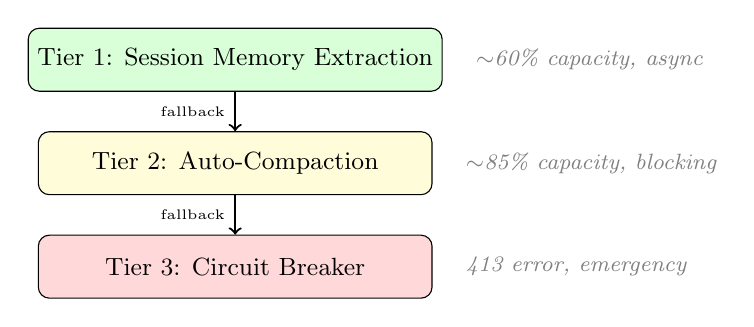
\begin{tikzpicture}[
  node distance=0.8cm,
  tier/.style={rectangle, draw, rounded corners, minimum width=5cm, minimum height=0.8cm, text centered, font=\small},
  arrow/.style={->, thick},
  label/.style={font=\footnotesize\itshape, text=gray}
]
\node[tier, fill=green!15] (t1) {Tier 1: Session Memory Extraction};
\node[label, right=0.3cm of t1] {$\sim$60\% capacity, async};
\node[tier, fill=yellow!15, below=0.5cm of t1] (t2) {Tier 2: Auto-Compaction};
\node[label, right=0.3cm of t2] {$\sim$85\% capacity, blocking};
\node[tier, fill=red!15, below=0.5cm of t2] (t3) {Tier 3: Circuit Breaker};
\node[label, right=0.3cm of t3] {413 error, emergency};
\draw[arrow] (t1) -- (t2) node[midway, left, font=\tiny]{fallback};
\draw[arrow] (t2) -- (t3) node[midway, left, font=\tiny]{fallback};
\end{tikzpicture}
\caption{Three-tier context management. Tiers are activated progressively as context pressure increases.}
\label{fig:context-mgmt}
\end{figure}

% ─────────────────────────────────────────────────────────────
\section{Multi-Layer Permission Architecture}
% ─────────────────────────────────────────────────────────────

\subsection{Design Philosophy}

Agent safety requires balancing autonomy (to reduce user friction) with oversight (to prevent destructive actions). Claude Code implements a \emph{multi-layer permission architecture} that applies different scrutiny levels depending on the estimated risk of a proposed action.

\subsection{Permission Modes}

The system supports three top-level permission modes, configurable globally or per-tool:
\begin{itemize}
  \item \textbf{\texttt{default}}: The agent may read files, run safe commands, and search without confirmation, but must confirm destructive or irreversible actions.
  \item \textbf{\texttt{bypass}}: All tool calls are allowed without confirmation. Intended for CI/CD pipelines and automated workflows.
  \item \textbf{\texttt{auto}}: An ML-based classifier determines whether each action requires confirmation.
\end{itemize}

\subsection{Five-Layer Decision Pipeline}

For each tool call, permission resolution proceeds through up to five layers (Figure~\ref{fig:permission}):

\paragraph{Layer 1: Input Validation.} The tool's input schema is validated via Zod before any permission check. Malformed inputs are rejected immediately.

\paragraph{Layer 2: Hook Pre-screening.} User-defined hooks (shell commands registered in \texttt{settings.json}) are executed synchronously. A hook exit code of 2 blocks the tool call with a user-visible message; exit code 0 allows unconditional execution.

\paragraph{Layer 3: ML Bash Classifier.} For \texttt{BashTool} specifically, an ML-based classifier analyzes the command string and classifies it into risk categories: \textit{safe} (read-only operations), \textit{caution} (file modifications), \textit{dangerous} (irreversible operations such as \texttt{rm -rf}), or \textit{network} (outbound connections). This classifier is implemented as a fine-tuned model call and its predictions are used to set the initial permission determination.

\paragraph{Layer 4: Persistent Rule Matching.} Approved and denied rules are persisted to \texttt{\textasciitilde/.claude/settings.json}. Before prompting the user, the system checks whether a matching rule already exists (using tool name and input pattern matching). If a matching allow rule exists, the call proceeds; if a deny rule matches, it is blocked.

\paragraph{Layer 5: Interactive Dialog.} If no cached rule applies, the user is presented with an interactive terminal dialog showing the full tool call parameters. The user can: (a) Allow once, (b) Allow always (persists a rule), (c) Deny once, or (d) Deny always (persists a rule).

\begin{figure}[t]
\centering
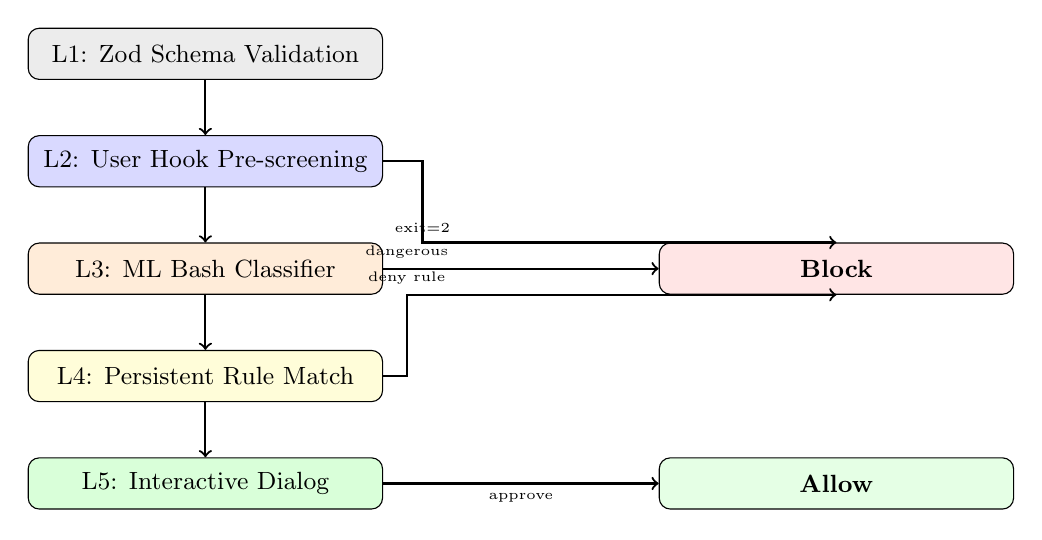
\begin{tikzpicture}[
  node distance=0.7cm,
  layer/.style={rectangle, draw, rounded corners, minimum width=4.5cm, minimum height=0.65cm, text centered, font=\small},
  decision/.style={diamond, draw, font=\tiny, aspect=3, minimum width=2.5cm},
  arrow/.style={->, thick}
]
\node[layer, fill=gray!15] (l1) {L1: Zod Schema Validation};
\node[layer, fill=blue!15, below=of l1] (l2) {L2: User Hook Pre-screening};
\node[layer, fill=orange!15, below=of l2] (l3) {L3: ML Bash Classifier};
\node[layer, fill=yellow!15, below=of l3] (l4) {L4: Persistent Rule Match};
\node[layer, fill=green!15, below=of l4] (l5) {L5: Interactive Dialog};
\node[layer, fill=red!10, right=3.5cm of l3] (block) {\textbf{Block}};
\node[layer, fill=green!10, right=3.5cm of l5] (allow) {\textbf{Allow}};
\draw[arrow] (l1) -- (l2);
\draw[arrow] (l2) -- (l3);
\draw[arrow] (l3) -- (l4);
\draw[arrow] (l4) -- (l5);
\draw[arrow] (l2.east) -- ++(0.5,0) |- node[above, font=\tiny]{exit=2} (block.north);
\draw[arrow] (l3.east) -- ++(0.3,0) |- node[above, font=\tiny]{dangerous} (block.west);
\draw[arrow] (l4.east) -- ++(0.3,0) |- node[above, font=\tiny]{deny rule} (block.south);
\draw[arrow] (l5) -- node[below, font=\tiny]{approve} (allow);
\end{tikzpicture}
\caption{Five-layer permission decision pipeline. Each layer can independently block a tool call.}
\label{fig:permission}
\end{figure}

% ─────────────────────────────────────────────────────────────
\section{Coordinator/Worker Multi-Agent Orchestration}
% ─────────────────────────────────────────────────────────────

\subsection{Architecture}

Claude Code implements a hierarchical multi-agent system through two complementary mechanisms: the \texttt{AgentTool} (available to all agents) and the Coordinator mode (enabled for complex tasks requiring parallel sub-agents).

\subsection{AgentTool: Sub-agent Spawning}

\texttt{AgentTool} (in \texttt{src/tools/AgentTool/}) allows any agent to spawn a sub-agent with a specified task. Sub-agents receive:
\begin{itemize}
  \item An \textbf{isolated execution context}: a cloned snapshot of the parent's file cache and tool state at spawn time.
  \item A \textbf{frozen system prompt}: the sub-agent's system prompt is locked at spawn time and cannot be modified by the sub-agent itself.
  \item A \textbf{restricted tool set}: the Coordinator can whitelist/blacklist specific tools for sub-agents, hiding internal coordination machinery from worker agents.
  \item A \textbf{budget}: optional token budget and turn limit constraints.
\end{itemize}

Sub-agents report results via a structured XML notification format, allowing the parent to parse results programmatically:
\begin{lstlisting}[language=XML]
<result>
  <status>success|error|interrupted</status>
  <output>...</output>
  <files_modified>...</files_modified>
  <tools_used>...</tools_used>
</result>
\end{lstlisting}

\subsection{Coordinator Mode}

The Coordinator mode (\texttt{src/coordinator/coordinatorMode.ts}) is activated for complex tasks requiring parallel execution of multiple workstreams. The Coordinator agent:
\begin{enumerate}
  \item Decomposes the task into independent sub-tasks.
  \item Assigns sub-tasks to Worker agents (spawned via \texttt{AgentTool}).
  \item Monitors Worker progress via task status polling.
  \item Merges Worker outputs and resolves conflicts.
\end{enumerate}

A critical safety property is \textbf{context isolation}: each Worker operates on its own context window and cannot directly read or modify the Coordinator's or other Workers' contexts. Information flows only through explicit result reports, preventing context contamination and enabling parallel execution without race conditions.

\subsection{Built-in Agent Types}

The system predefines several specialized agent types (Table~\ref{tab:agent-types}), each configured with a tailored system prompt and tool set.

\begin{table}[t]
\centering
\caption{Built-in sub-agent types in Claude Code.}
\label{tab:agent-types}
\small
\begin{tabular}{lll}
\toprule
\textbf{Type} & \textbf{Available Tools} & \textbf{Primary Use} \\
\midrule
\texttt{general-purpose} & All & General sub-tasks \\
\texttt{Plan} & Read, Glob, Grep, WebSearch & Task planning \\
\texttt{Explore} & Read, Glob, Grep (no Edit/Write) & Codebase exploration \\
\texttt{claude-code-guide} & Glob, Grep, Read, WebFetch, WebSearch & Documentation queries \\
\texttt{statusline-setup} & Read, Edit & Config file modification \\
\bottomrule
\end{tabular}
\end{table}

% ─────────────────────────────────────────────────────────────
\section{Model Context Protocol Integration}
% ─────────────────────────────────────────────────────────────

\subsection{Overview}

The Model Context Protocol (MCP)~\cite{anthropic2024mcp} is an open standard for connecting LLMs to external data sources and tools. Claude Code implements a comprehensive MCP client layer in \texttt{src/services/mcp/} (22 files) that enables dynamic extension of the agent's capabilities at runtime.

\subsection{MCP Architecture in Claude Code}

The MCP integration layer provides:

\paragraph{Transport abstraction.} Three transport implementations are supported:
\begin{itemize}
  \item \textbf{stdio transport}: Spawns an MCP server as a child process and communicates via stdin/stdout.
  \item \textbf{SSE transport}: Connects to an HTTP server using Server-Sent Events.
  \item \textbf{In-process transport}: For first-party tools that are architecturally MCP-compatible but run in-process.
\end{itemize}

\paragraph{Dynamic tool discovery.} At session initialization, Claude Code queries each registered MCP server for its tool manifest (name, description, input schema). These tools are dynamically added to the agent's available tool set and included in the system prompt's tool reference section.

\paragraph{Schema translation.} MCP tool schemas (JSON Schema) are translated to Zod schemas for runtime validation. Tool results (text, images, embeddings) are normalized into the agent's internal result format.

\paragraph{Authentication.} The MCP layer supports OAuth 2.0 flows for servers requiring authentication, with credentials persisted to \texttt{\textasciitilde/.claude/mcp-credentials/}.

\subsection{First-Party MCP Tools}

Claude Code exposes its own capabilities as MCP tools, enabling external orchestrators (e.g., Claude Desktop) to invoke Claude Code as an MCP server. This bidirectional MCP architecture allows Claude Code to act simultaneously as an MCP client (consuming third-party tools) and an MCP server (exposing its capabilities to other systems).

% ─────────────────────────────────────────────────────────────
\section{Task Management System}
% ─────────────────────────────────────────────────────────────

Claude Code includes a persistent task management system that bridges the gap between long-horizon planning and immediate execution. Tasks are defined in \texttt{src/Task.ts} with the following schema:

\begin{lstlisting}[language=TypeScript]
interface Task {
  id: string;
  subject: string;
  description: string;
  status: "pending" | "in_progress" | "completed" | "blocked";
  owner: "claude" | "user";
  blockedBy?: string[];
  blocks?: string[];
  created: number;
  updated: number;
}
\end{lstlisting}

Five tool implementations (\texttt{TaskCreateTool}, \texttt{TaskUpdateTool}, \texttt{TaskGetTool}, \texttt{TaskListTool}, \texttt{TaskStopTool}) provide CRUD operations. Dependency tracking (\texttt{blockedBy}/\texttt{blocks}) allows the agent to reason about task ordering and prevent premature execution of dependent steps. Tasks are persisted to the session store and survive context compaction, providing a lightweight planning layer that survives context window management operations.

% ─────────────────────────────────────────────────────────────
\section{Additional Architectural Features}
% ─────────────────────────────────────────────────────────────

\subsection{Long-Term Memory (\texttt{memdir})}

Claude Code implements a file-based memory system in \texttt{src/memdir/} that persists information across sessions. Memory entries are stored as Markdown files with YAML frontmatter specifying type (\texttt{user}, \texttt{feedback}, \texttt{project}, \texttt{reference}), name, and description. A \texttt{MEMORY.md} index file is automatically loaded into every session's context, providing a lightweight retrieval mechanism. This is distinct from RAG-based approaches~\cite{lewis2020retrieval} in that it is \emph{agent-authored} (the agent decides what to remember) rather than document-indexed.

\subsection{Hook System}

User-defined hooks are shell commands registered in \texttt{settings.json} that execute at specific lifecycle events:
\begin{itemize}
  \item \texttt{PreToolUse}: Runs before a tool call; exit code 2 blocks execution.
  \item \texttt{PostToolUse}: Runs after a tool call completes.
  \item \texttt{Notification}: Runs when the agent sends a notification.
  \item \texttt{Stop}: Runs when the agent completes a task.
\end{itemize}
This provides an extensibility point analogous to Git hooks, enabling users to integrate Claude Code into existing workflows (e.g., logging, automatic formatting, CI integration) without modifying the agent itself.

\subsection{Skill System}

Skills are pre-authored prompt templates stored as Markdown files in \texttt{\textasciitilde/.claude/skills/}. The \texttt{SkillTool} loads and expands skill templates at runtime, injecting them into the conversation as if the user had typed the expanded prompt. This enables reusable, shareable agent behaviors --- analogous to macros or functions in traditional programming.

\subsection{Voice Mode}

A push-to-talk voice interface is implemented in \texttt{src/voice/}, using browser/system audio APIs for capture and the Whisper API for transcription. This mode uses the same underlying agentic loop; voice input is transcribed and injected as text into the standard processing pipeline.

\subsection{Vim Keybindings}

The terminal UI (\texttt{src/vim/}) supports Vim-style modal editing for the input field (Normal/Insert/Visual modes), implemented as a custom keymap layer on top of Ink's input handling. This reflects a design philosophy of meeting developers in their existing workflows.

% ─────────────────────────────────────────────────────────────
\section{Design Principles and Lessons Learned}
% ─────────────────────────────────────────────────────────────

Our analysis of Claude Code's architecture yields several design principles that we believe are broadly applicable to the construction of production agentic systems.

\paragraph{P1: API-turn granularity over user-turn granularity.}
Organizing the inner loop around API turns (rather than user turns) enables complex multi-step tasks within a single user interaction, decoupling the user experience from the inference cadence. This is particularly important for tasks with unpredictable depth.

\paragraph{P2: Ordered output buffering for concurrent tools.}
Parallel tool execution is essential for latency, but LLM APIs impose ordering semantics on tool results. An ordered output buffer allows maximum concurrency while preserving these semantics, avoiding subtle context corruption bugs.

\paragraph{P3: Memory-first context management.}
Proactive, asynchronous session memory extraction is preferable to reactive summarization because it (a) incurs zero latency on the critical path and (b) preserves high-fidelity information while there is still context budget to do so. Reactive compaction should be a fallback, not the primary strategy.

\paragraph{P4: Progressive permission scrutiny.}
A multi-layer permission system can achieve both low friction (for safe operations) and high safety (for dangerous operations) by applying scrutiny proportional to estimated risk. ML-based pre-screening reduces the frequency of user interruptions without sacrificing oversight.

\paragraph{P5: Context isolation as a first-class property of multi-agent systems.}
In multi-agent systems, strict context isolation between agents (with information flowing only through explicit result channels) prevents context contamination and enables safe parallel execution. Systems that allow implicit context sharing risk subtle coordination failures.

\paragraph{P6: Persistent declarative rules over repeated interactive confirmation.}
Allowing users to encode decisions as persistent rules (rather than re-confirming identical actions repeatedly) dramatically reduces friction while maintaining user control. The ``allow always / deny always'' mechanism is a simple but highly effective UX pattern.

% ─────────────────────────────────────────────────────────────
\section{Discussion}
% ─────────────────────────────────────────────────────────────

\subsection{Limitations and Open Problems}

\paragraph{Context management quality.}
While the three-tier context strategy prevents hard failures, the quality of compacted summaries remains a function of the summarization model's capabilities. Information loss during compaction can degrade agent performance on tasks requiring recall of earlier events. Principled methods for \emph{selective} context retention (e.g., importance-weighted retention~\cite{liu2023lost}) remain an open research problem.

\paragraph{ML classifier reliability.}
The Bash risk classifier operates on command strings without executing them, making it vulnerable to obfuscation (e.g., variable interpolation, heredocs). A more robust approach might combine static analysis with dynamic sandboxing~\cite{ruan2023identifying}.

\paragraph{Multi-agent conflict resolution.}
The Coordinator/Worker model assumes that sub-tasks can be executed independently. When sub-tasks have implicit dependencies (e.g., both modifying the same file), the system may produce conflicting results that require post-hoc reconciliation. Formal dependency analysis at the task decomposition stage is an interesting future direction.

\paragraph{Memory retrieval at scale.}
The current \texttt{MEMORY.md} index approach loads all memory entries into context at session start. As the number of entries grows, this becomes increasingly costly. Vector-based retrieval~\cite{lewis2020retrieval} or hierarchical memory organization could address this.

\subsection{Broader Implications}

Claude Code's architecture illustrates a broader trend: the most significant engineering challenges in LLM agents are not in model capability, but in the \emph{system design} that wraps model capability. Context management, permission architecture, multi-agent coordination, and extensibility infrastructure collectively determine whether an agent is useful in practice. We hope this analysis contributes to a shared vocabulary for reasoning about these challenges.

% ─────────────────────────────────────────────────────────────
\section{Conclusion}
% ─────────────────────────────────────────────────────────────

We have presented a systematic architectural analysis of Claude Code v2.1.88, identifying five core technical contributions: (1) a streaming agentic loop with API-turn granularity and ordered-buffered concurrent tool execution; (2) a three-tier context management strategy combining proactive memory extraction, auto-compaction, and circuit-breaker recovery; (3) a five-layer permission architecture integrating ML-based risk classification with persistent declarative rules; (4) a Coordinator/Worker multi-agent system with strict context isolation; and (5) a bidirectional MCP integration layer enabling dynamic tool extension.

These contributions collectively represent a coherent and pragmatic answer to the core engineering challenges of production LLM agent systems. The design principles we extract from this analysis --- API-turn granularity, ordered output buffering, memory-first context management, progressive permission scrutiny, context isolation, and persistent declarative rules --- provide a useful vocabulary for the design and evaluation of future agentic systems.

% ─────────────────────────────────────────────────────────────
\begin{ack}
Omitted for double-blind review.
\end{ack}

% ─────────────────────────────────────────────────────────────
\bibliographystyle{plain}
\bibliography{references}

\begin{thebibliography}{99}

\bibitem{anthropic2024claudecode}
Anthropic.
\newblock {Claude Code}: Agentic coding in your terminal.
\newblock \url{https://docs.anthropic.com/en/docs/claude-code}, 2024.

\bibitem{anthropic2024mcp}
Anthropic.
\newblock Model context protocol.
\newblock \url{https://modelcontextprotocol.io}, 2024.

\bibitem{autogpt2023}
Significant Gravitas.
\newblock {AutoGPT}: An autonomous {GPT-4} experiment.
\newblock \url{https://github.com/Significant-Gravitas/AutoGPT}, 2023.

\bibitem{chen2021evaluating}
Mark Chen, Jerry Tworek, Heewoo Jun, et al.
\newblock Evaluating large language models trained on code.
\newblock \textit{arXiv preprint arXiv:2107.03374}, 2021.

\bibitem{cognition2024devin}
Cognition AI.
\newblock Introducing {Devin}, the first {AI} software engineer.
\newblock \url{https://www.cognition.ai/blog/introducing-devin}, 2024.

\bibitem{hong2023metagpt}
Sirui Hong, Mingchen Zhuge, Jonathan Chen, et al.
\newblock {MetaGPT}: Meta programming for a multi-agent collaborative framework.
\newblock \textit{arXiv preprint arXiv:2308.00352}, 2023.

\bibitem{ink2023}
Vadim Demedes.
\newblock {Ink}: React for interactive command-line apps.
\newblock \url{https://github.com/vadimdemedes/ink}, 2023.

\bibitem{langchain2022}
Harrison Chase.
\newblock {LangChain}: Building applications with {LLMs} through composability.
\newblock \url{https://github.com/langchain-ai/langchain}, 2022.

\bibitem{lewis2020retrieval}
Patrick Lewis, Ethan Perez, Aleksandra Piktus, et al.
\newblock Retrieval-augmented generation for knowledge-intensive {NLP} tasks.
\newblock In \textit{NeurIPS}, 2020.

\bibitem{liu2023lost}
Nelson F.\ Liu, Kevin Lin, John Hewitt, et al.
\newblock Lost in the middle: How language models use long contexts.
\newblock \textit{Transactions of the ACL}, 2024.

\bibitem{nakajima2023babyagi}
Yohei Nakajima.
\newblock {BabyAGI}: Task-driven autonomous agent.
\newblock \url{https://github.com/yoheinakajima/babyagi}, 2023.

\bibitem{park2023generative}
Joon Sung Park, Joseph C.\ O'Brien, Carrie J.\ Cai, et al.
\newblock Generative agents: Interactive simulacra of human behavior.
\newblock In \textit{UIST}, 2023.

\bibitem{ruan2023identifying}
Yangjun Ruan, Honghua Dong, Andrew Wang, et al.
\newblock Identifying the risks of {LM} agents with an {LM}-emulated sandbox.
\newblock \textit{arXiv preprint arXiv:2309.15817}, 2023.

\bibitem{schick2023toolformer}
Timo Schick, Jane Dwivedi-Yu, Roberto Dessi, et al.
\newblock Toolformer: Language models can teach themselves to use tools.
\newblock In \textit{NeurIPS}, 2023.

\bibitem{shi2024ehragent}
Wenqi Shi, Runlong Yu, Shengchao Liu, et al.
\newblock {EHRAgent}: Code empowers large language models for few-shot complex tabular reasoning on electronic health records.
\newblock \textit{arXiv preprint arXiv:2401.07128}, 2024.

\bibitem{shinn2023reflexion}
Noah Shinn, Federico Cassano, Ashwin Gopinath, et al.
\newblock Reflexion: Language agents with verbal reinforcement learning.
\newblock In \textit{NeurIPS}, 2023.

\bibitem{wang2023plan}
Lei Wang, Wanyu Xu, Yihuai Lan, et al.
\newblock Plan-and-solve prompting: Improving zero-shot chain-of-thought reasoning by large language models.
\newblock In \textit{ACL}, 2023.

\bibitem{wang2024openhands}
Xingyao Wang, Boxuan Li, Yufan Song, et al.
\newblock {OpenHands}: An open platform for {AI} software developers as generalist agents.
\newblock \textit{arXiv preprint arXiv:2407.16741}, 2024.

\bibitem{wei2022chain}
Jason Wei, Xuezhi Wang, Dale Schuurmans, et al.
\newblock Chain-of-thought prompting elicits reasoning in large language models.
\newblock In \textit{NeurIPS}, 2022.

\bibitem{wu2023autogen}
Qingyun Wu, Gagan Bansal, Jieyu Zhang, et al.
\newblock {AutoGen}: Enabling next-gen {LLM} applications via multi-agent conversation.
\newblock \textit{arXiv preprint arXiv:2308.08155}, 2023.

\bibitem{yang2024sweagent}
John Yang, Carlos E.\ Jimenez, Alexander Wettig, et al.
\newblock {SWE-agent}: Agent-computer interfaces enable automated software engineering.
\newblock In \textit{NeurIPS}, 2024.

\bibitem{yao2022react}
Shunyu Yao, Jeffrey Zhao, Dian Yu, et al.
\newblock {ReAct}: Synergizing reasoning and acting in language models.
\newblock In \textit{ICLR}, 2023.

\bibitem{zhang2024survey}
Jiawei Zhang, Haipeng Luo, Taesoo Kim, and Bang Liu.
\newblock A survey on long text modeling with transformers.
\newblock \textit{arXiv preprint arXiv:2302.14802}, 2024.

\end{thebibliography}

% ─────────────────────────────────────────────────────────────
\appendix
% ─────────────────────────────────────────────────────────────
\section{Tool Taxonomy}
\label{app:tools}

Table~\ref{tab:tools} provides a complete taxonomy of the 40+ tools available in Claude Code, organized by category.

\begin{table}[h]
\centering
\caption{Complete tool taxonomy in Claude Code v2.1.88.}
\label{tab:tools}
\small
\begin{tabular}{lll}
\toprule
\textbf{Category} & \textbf{Tool} & \textbf{Concurrent?} \\
\midrule
\multirow{3}{*}{File I/O}
  & \texttt{FileReadTool} & Yes \\
  & \texttt{FileWriteTool} & No \\
  & \texttt{FileEditTool} & No \\
\midrule
\multirow{2}{*}{Code Search}
  & \texttt{GlobTool} & Yes \\
  & \texttt{GrepTool} & Yes \\
\midrule
System Execution
  & \texttt{BashTool} & No \\
\midrule
\multirow{2}{*}{Web}
  & \texttt{WebFetchTool} & Yes \\
  & \texttt{WebSearchTool} & Yes \\
\midrule
\multirow{4}{*}{Task Management}
  & \texttt{TaskCreateTool} & No \\
  & \texttt{TaskUpdateTool} & No \\
  & \texttt{TaskGetTool} & Yes \\
  & \texttt{TaskListTool} & Yes \\
\midrule
\multirow{2}{*}{Sub-agent}
  & \texttt{AgentTool} & Yes \\
  & \texttt{SkillTool} & Yes \\
\midrule
\multirow{2}{*}{Dev Environment}
  & \texttt{NotebookEditTool} & No \\
  & \texttt{LSPTool} & Yes \\
\midrule
\multirow{2}{*}{Git / Worktree}
  & \texttt{EnterWorktreeTool} & No \\
  & \texttt{ExitWorktreeTool} & No \\
\midrule
\multirow{3}{*}{Planning}
  & \texttt{TodoWriteTool} & No \\
  & \texttt{EnterPlanModeTool} & No \\
  & \texttt{ExitPlanModeTool} & No \\
\midrule
\multirow{2}{*}{Automation}
  & \texttt{ScheduleCronTool} & No \\
  & \texttt{RemoteTriggerTool} & No \\
\midrule
User Interaction
  & \texttt{AskUserQuestionTool} & No \\
\midrule
MCP
  & \texttt{MCPTool} (dynamic) & Varies \\
\bottomrule
\end{tabular}
\end{table}

\section{Slash Command Taxonomy}
\label{app:commands}

Claude Code exposes approximately 87 slash commands. Key commands by category:

\begin{itemize}
  \item \textbf{Git/Code}: \texttt{/commit}, \texttt{/commit-push-pr}, \texttt{/review}
  \item \textbf{Session}: \texttt{/resume}, \texttt{/session}, \texttt{/clear}
  \item \textbf{Memory}: \texttt{/memory}, \texttt{/compact}
  \item \textbf{Config}: \texttt{/config}, \texttt{/permissions}, \texttt{/theme}
  \item \textbf{Integrations}: \texttt{/mcp}, \texttt{/desktop}, \texttt{/skills}
  \item \textbf{UI}: \texttt{/vim}, \texttt{/voice}, \texttt{/copy}
  \item \textbf{Help}: \texttt{/help}, \texttt{/doctor}
  \item \textbf{Hidden}: \texttt{/btw}, \texttt{/stickers}
\end{itemize}

\end{document}
